\documentclass{article}
\usepackage{tikz}
\usetikzlibrary{arrows.meta}

\tikzset{
  database/.pic = {
    \draw (0,0) ellipse (1.25 and 0.5);
    \draw (-1.25,0) -- (-1.25,-3.5);
    \draw (-1.25,-3.5) arc (180:360:1.25 and 0.5);
    %\draw [dashed] (-1.25,-3.5) arc (180:360:1.25 and -0.5);
    \draw (1.25,-3.5) -- (1.25, 0);
    \fill [gray,opacity=0.5] (-1.25,0) -- (-1.25,-3.5) arc (180:360:1.25 and 0.5) -- (1.25,0) arc (0:180:1.25 and -0.5);
  }
}

\begin{document}
\begin{figure}
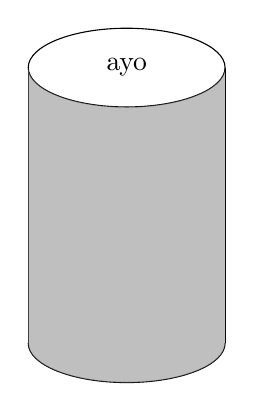
\begin{tikzpicture}
  \path (0,0) pic{database};
  \node (sldb) at (0,0) {ayo};

%  \node (sk) at (0,2) {$P_{sk}$};
%  \node [below=2cm] (msg) at (sk) {$\{ep, sl, ep_{seed}, S_{pk}\}$};
%  \node [right=1cm] (vrf) at (sk) {VRF};
%  \node [right=1cm] (eval) at (vrf) {$VRF_{eval}$};
%  \node [circle,below=1cm,right=1cm] (check) at (eval) {check};
%  \node [below=1cm,left=0.5cm] (threshold) at (check) {$T_{ep}^S$};
%  \node [below=1cm,right=0.5cm] (pk) at (check) {$P_{pk}$};
%  \node [right=1cm] (condition) at (check) {True/False};
%
%  \draw [thick,-Latex] (sk) -- (vrf);
%  \draw [thick,-Latex] (msg) -- (vrf);
%  \draw [thick,-Latex] (vrf) -- (eval);
%  \draw [thick,-Latex] (eval) -- (check);
%  \draw [thick,-Latex] (msg) -- (check);
%  \draw [thick,-Latex] (threshold) -- (check);
%  \draw [thick,-Latex] (pk) -- (check);
%  \draw [thick,-Latex] (check) -- (condition);
\end{tikzpicture}
\end{figure}
\end{document}
